\documentclass{article}

\usepackage[12pt]{extsizes}
\usepackage[T2A]{fontenc}
\usepackage[utf8]{inputenc}
\usepackage[english, russian]{babel}

\usepackage{mathrsfs}
\usepackage[dvipsnames]{xcolor}

\usepackage{amsmath}
\usepackage{amssymb}
\usepackage{amsthm}
\usepackage{indentfirst}
\usepackage{amsfonts}
\usepackage{enumitem}
\usepackage{graphics}
\usepackage{tikz}
\usepackage{tabu}
\usepackage{diagbox}
\usepackage{hyperref}
\usepackage{mathtools}
\usepackage{ucs}
\usepackage{lipsum}
\usepackage{geometry} % Меняем поля страницы
\usepackage{fancyhdr} % Headers and footers
\newcommand{\range}{\mathrm{range}}
\newcommand{\dom}{\mathrm{dom}}
\newcommand{\N}{\mathbb{N}}
\newcommand{\R}{\mathbb{R}}
\newcommand{\E}{\mathbb{E}}
\newcommand{\D}{\mathbb{D}}
\newcommand{\M}{\mathcal{M}}
\newcommand{\Prime}{\mathbb{P}}
\newcommand{\A}{\mathbb{A}}
\newcommand{\Q}{\mathbb{Q}}
\newcommand{\Z}{\mathbb{Z}}
\newcommand{\F}{\mathbb{F}}
\newcommand{\CC}{\mathbb{C}}

\DeclarePairedDelimiter\abs{\lvert}{\rvert}
\DeclarePairedDelimiter\floor{\lfloor}{\rfloor}
\DeclarePairedDelimiter\ceil{\lceil}{\rceil}
\DeclarePairedDelimiter\lr{(}{)}
\DeclarePairedDelimiter\set{\{}{\}}
\DeclarePairedDelimiter\norm{\|}{\|}

\renewcommand{\labelenumi}{(\alph{enumi})}

\newcommand{\smallindent}{
    \geometry{left=1cm}% левое поле
    \geometry{right=1cm}% правое поле
    \geometry{top=1.5cm}% верхнее поле
    \geometry{bottom=1cm}% нижнее поле
}

\newcommand{\header}[3]{
    \pagestyle{fancy} % All pages have headers and footers
    \fancyhead{} % Blank out the default header
    \fancyfoot{} % Blank out the default footer
    \fancyhead[L]{#1}
    \fancyhead[C]{#2}
    \fancyhead[R]{#3}
}

\newcommand{\dividedinto}{
    \,\,\,\vdots\,\,\,
}

\newcommand{\littletaller}{\mathchoice{\vphantom{\big|}}{}{}{}}

\newcommand\restr[2]{{
    \left.\kern-\nulldelimiterspace % automatically resize the bar with \right
    #1 % the function
    \littletaller % pretend it's a little taller at normal size
    \right|_{#2} % this is the delimiter
}}

\DeclareGraphicsExtensions{.pdf,.png,.jpg}

\newenvironment{enumerate_boxed}[1][enumi]{\begin{enumerate}[label*=\protect\fbox{\arabic{#1}}]}{\end{enumerate}}



\smallindent

\header{ЦРОД $\bullet$ Математика}{\textit{Методы}}{ЛФМШ 2022}

%----------------------------------------------------------------------------------------

\begin{document}
    \large

    \begin{center}
        \textbf{Оценка+пример}
    \end{center}

    \textit{Задача:} Какое наибольшее число трёхклеточных уголков можно вырезать из клетчатого квадрата $8 \times 8$?

    \textit{Решение:} В квадрате $8 \time 8=64$ клетки.
    Поэтому вырезать $22$ и более уголков не получится: ведь тогда суммарное число клеток в них будет не меньше $22\cdot 3 = 66$.
    Значит, число уголков не больше $21$ (\textit{оценка}).
    Вырезать $21$ уголок можно - \textit{пример}~\ref{ris:1}.
    Следовательно, наибольшее возможное количество уголков равно $21$.

    \begin{figure}[h]
        \begin{center}
            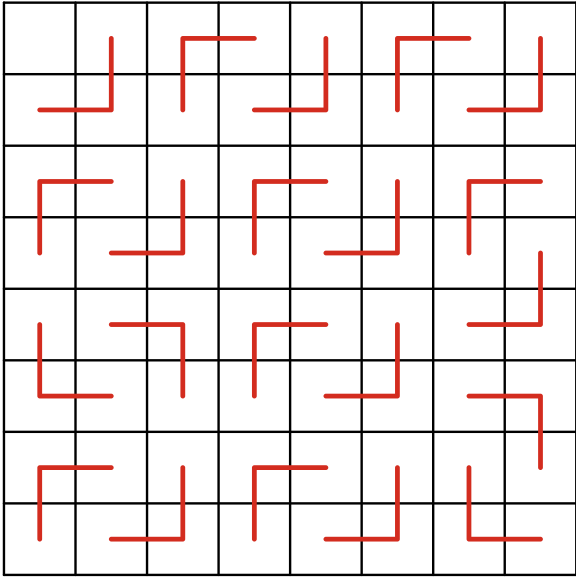
\includegraphics[width=0.3\linewidth]{primer}
            \caption{Пример} %% подпись к рисунку
            \label{ris:1} %% метка рисунка для ссылки на него
        \end{center}
    \end{figure}

    Логика рассуждения ясна: мы показали, что количество уголков не превосходит числа $21$
    (\textit{оценка}) и иногда ему равно (\textit{пример}). Значит, $21$ и есть максимум числа уголков.


    \begin{enumerate_boxed}
        \item Какое наименьшее число ладей могут побить всю шахматную доску?

        \item Найдите наименьшее натуральное число кратное $5$, сумма цифр которого равна $25$.

        \item Какое наибольшее число трёхклеточных уголков можно вырезать из клетчатого прямоугольника $5 \times 7$?

        \item У вас есть три котлеты и две сковороды.
        Каждая сторона котлеты жарится одну минуту.
        На одну сковороду одновременно помещается лишь одна котлета.
        За какое наименьшее время можно пожарить все котлеты с обеих сторон?

        \item Найдите наибольшее натуральное число, которое невозможно представить в виде суммы двух составных чисел.

        \item Каково наименьшее натуральное $n$ такое, что $n!$ делится на 18, на 19, на 20 и на 21?

        \item Какое наименьшее число клеточек на доске 8×8 можно закрасить в чёрный цвет так, чтобы была хотя бы одна закрашенная клетка:

        \begin{enumerate}
            \item[a)] в любом квадратике $2\times2$?
            \item[б)] в любом уголке из трёх клеточек?
        \end{enumerate}

        \item Сложите квадрат из наименьшего возможного количества трёхклеточных уголков.

        \item Белоснежка вошла в комнату, где вокруг круглого стола стояло 30 стульев.
        На некоторых из стульев сидели гномы.
        Оказалось, что Белоснежка не может сесть так, чтобы рядом с ней никто не сидел.
        Какое наименьшее число гномов могло быть за столом?

        \item $48$ кузнецов должны подковать $60$ лошадей.
        Какое наименьшее время они затратят на работу, если каждый кузнец тратит на одну подкову пять минут?
        (Лошадь не может стоять на двух ногах.)

        \item Какое наименьшее количество трехклеточных уголков можно разместить в квадрате $8 \times 8$ так, чтобы в этот квадрат больше нельзя было поместить ни одного такого уголка?

        \item Поле представляет собой клетчатый квадрат $41 \times 41$, в одной из клеток которого замаскирован танк.
        Истребитель за один выстрел обстреливает одну клетку.
        Если произошло попадание, танк переползает на соседнюю по стороне клетку поля, если нет – остаётся на месте.
        При этом после выстрела пилот истребителя не знает, произошло ли попадание.
        Для уничтожения танка надо попасть в него два раза.
        Каким наименьшим числом выстрелов можно обойтись для того, чтобы гарантировать, что танк уничтожен?


    \end{enumerate_boxed}
\end{document}